\documentclass[12pt]{article} % use larger type; default would be 10pt
\usepackage[utf8]{inputenc}
\usepackage{geometry} % to change the page dimensions
\geometry{letterpaper} 
\geometry{letterpaper} % or letterpaper (US) or a5paper or....
% \geometry{margin=2in} % for example, change the margins to 2 inches all round
% \geometry{landscape} % set up the page for landscape
%   read geometry.pdf for detailed page layout information
\usepackage{graphicx} % support the \includegraphics command 
\usepackage{booktabs} % for much better looking tables
\usepackage{array} % for arrays
\usepackage{verbatim} % adds environment for commenting out blocks of text
\usepackage{subfig}\usepackage{eqnarray, amsmath}
\usepackage[makeroom]{cancel}
\usepackage{sidecap}
\usepackage{fancyhdr} % This should be set AFTER setting up the page geometry
\pagestyle{fancy} % options: empty , plain , fancy
\renewcommand{\headrulewidth}{0pt} % customise the layout...
\lhead{}\chead{}\rhead{}
\lfoot{}\cfoot{\thepage}\rfoot{}
%%% SECTION TITLE APPEARANCE
\usepackage{sectsty}
\allsectionsfont{\sffamily\mdseries\upshape} % (See the fntguide.pdf for font help)
% (This matches ConTeXt defaults)
%%% ToC (table of contents) APPEARANCE
\usepackage[nottoc,notlof,notlot]{tocbibind} % Put the bibliography in the ToC
\usepackage[titles,subfigure]{tocloft} % Alter the style of the Table of Contents
\renewcommand{\cftsecfont}{\rmfamily\mdseries\upshape}
\renewcommand{\cftsecpagefont}{\rmfamily\mdseries\upshape} % No bold!
\usepackage{pdfpages}
%\includepdf[pages={1}]{myfile.pdf}
\usepackage{listings}
\usepackage{color} %red, green, blue, yellow, cyan, magenta, black, white
\definecolor{mygreen}{RGB}{28,172,0} % color values Red, Green, Blue
\definecolor{mylilas}{RGB}{170,55,241}



\title{{\bf {Project 1}}}
\author{Abraham Jacob Reines}
\date{March 27, 2022} % Activate to display a given date or no date (if empty),
         % otherwise the current date is printed 
\begin{document}
\maketitle
\hfill
\newpage

\section{Problem 1}
{\bf{Problem:}}
Write an algorithm called factors that takes a positive integer n and outputs the number of factors for n. 

\subsection{Solution:}


\lstset{language=Matlab,%
    %basicstyle=\color{red},
    breaklines=true,%
    morekeywords={matlab2tikz},
    keywordstyle=\color{blue},%
    morekeywords=[2]{1}, keywordstyle=[2]{\color{black}},
    identifierstyle=\color{black},%
    stringstyle=\color{mylilas},
    commentstyle=\color{mygreen},%
    showstringspaces=false,%without this there will be a symbol in the places where there is a space
    numbers=left,%
    numberstyle={\tiny \color{black}},% size of the numbers
    numbersep=9pt, % this defines how far the numbers are from the text
    emph=[1]{for,end,break},emphstyle=[1]\color{red}, %some words to emphasise
    %emph=[2]{word1,word2}, emphstyle=[2]{style},    
}


\section*{Matlab Code}

\lstinputlisting{factors.m}

%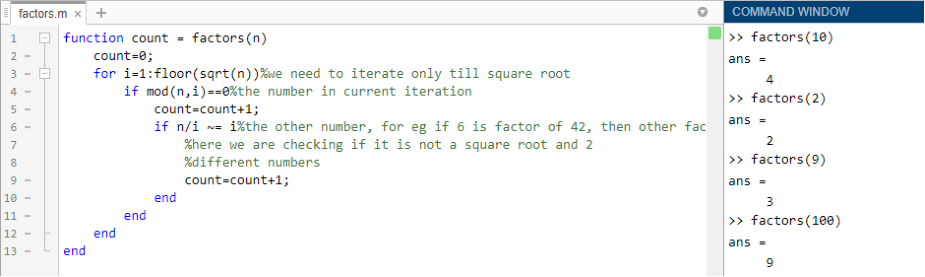
\includepdf[pages={1}]{Picture1.pdf}

\subsection{Description of solution:}
The first if-statement sets a ceiling (floor) for the iteration to stop at the square of the positive integer.  The second if-statement applies a mod function as discussed in class.  The third if-statement checks the other number, for example, when dividing 42/6 = 7, we are checking if 42 is not a square root and 2 different numbers. 

\subsection{Results and Conclusions:}
All results from factors inputs produced reasonable factors! This indicates the algorithm is performing within constraints, such as positive integer inputs.  
Factors(10) = 4.

\hfill
\newpage

\section {Problem 2}
{\bf{Problem: }}
Which number less than five hundred thousand has the most factors? Write a loop that calls factors.

\subsection{Description of solution:}
An if-statement with 3 variables utilized in conjunction with factors from Problem 1 produces a number less than 500,000 with the most factors possible.  The if-statement sets a ceiling for 500000 and uses the function to find the integer with the most factors.

\subsection{Results and Conclusions:}
All results from if-statement inputs produced reasonable output responses! This indicates the algorithm is performing properly for the problem.  
Answer: the number less than 500,000 with the most factors is 498,960.

\subsection{Solution:}

\lstset{language=Matlab,%
    %basicstyle=\color{red},
    breaklines=true,%
    morekeywords={matlab2tikz},
    keywordstyle=\color{blue},%
    morekeywords=[2]{1}, keywordstyle=[2]{\color{black}},
    identifierstyle=\color{black},%
    stringstyle=\color{mylilas},
    commentstyle=\color{mygreen},%
    showstringspaces=false,%without this there will be a symbol in the places where there is a space
    numbers=left,%
    numberstyle={\tiny \color{black}},% size of the numbers
    numbersep=9pt, % this defines how far the numbers are from the text
    emph=[1]{for,end,break},emphstyle=[1]\color{red}, %some words to emphasise
    %emph=[2]{word1,word2}, emphstyle=[2]{style},    
}


\section*{Matlab Code}

\lstinputlisting{factors50000test.m}

\hfill
\newpage

\section {Problem 3}
{\bf{Problem: }}
Which number less than five hundred thousand has the most factors? Write a loop that calls factors.

\subsection{Solution:}

\lstset{language=Matlab,%
    %basicstyle=\color{red},
    breaklines=true,%
    morekeywords={matlab2tikz},
    keywordstyle=\color{blue},%
    morekeywords=[2]{1}, keywordstyle=[2]{\color{black}},
    identifierstyle=\color{black},%
    stringstyle=\color{mylilas},
    commentstyle=\color{mygreen},%
    showstringspaces=false,%without this there will be a symbol in the places where there is a space
    numbers=left,%
    numberstyle={\tiny \color{black}},% size of the numbers
    numbersep=9pt, % this defines how far the numbers are from the text
    emph=[1]{for,end,break},emphstyle=[1]\color{red}, %some words to emphasise
    %emph=[2]{word1,word2}, emphstyle=[2]{style},    
}


\section*{Matlab Code}

\lstinputlisting{prime.m}
\lstinputlisting{prime2.m}

%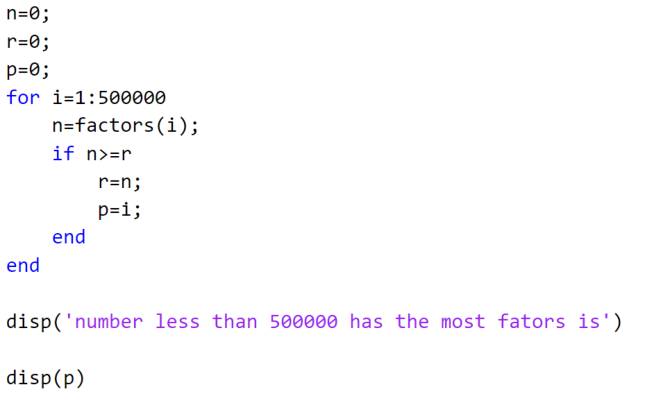
\includepdf[pages={1}]{Picture2.pdf}

\subsection{Description of solution:}
Two different functions solve this problem.  One utilizes a combination of if and else-statements.  The if-statement is crucial to obtaining the prime from factors. 
The bottom algorithm is a function more similar to Problem 1.

\subsection{Results and Conclusions:}
All results from prime function inputs produced accurate output responses! This indicates the algorithm is performing properly for the problem constraints.

\section {Problem 4}
{\bf{Problem: }}
Using the function from Problem 3, what is the 6000th prime?

\subsection{Description of solution:}
Utilizing the prime function from Problem 3, add a while loop to find the 6000th prime

\subsection{Results and Conclusions:}
All results from prime function inputs produced accurate output responses! This indicates the algorithm is performing properly for the problem constraints.  
The 6000th prime is 59,359.

\hfill
\newpage

\subsection{Solution:}

\lstset{language=Matlab,%
    %basicstyle=\color{red},
    breaklines=true,%
    morekeywords={matlab2tikz},
    keywordstyle=\color{blue},%
    morekeywords=[2]{1}, keywordstyle=[2]{\color{black}},
    identifierstyle=\color{black},%
    stringstyle=\color{mylilas},
    commentstyle=\color{mygreen},%
    showstringspaces=false,%without this there will be a symbol in the places where there is a space
    numbers=left,%
    numberstyle={\tiny \color{black}},% size of the numbers
    numbersep=9pt, % this defines how far the numbers are from the text
    emph=[1]{for,end,break},emphstyle=[1]\color{red}, %some words to emphasise
    %emph=[2]{word1,word2}, emphstyle=[2]{style},    
}


\lstinputlisting{prime3.m}

%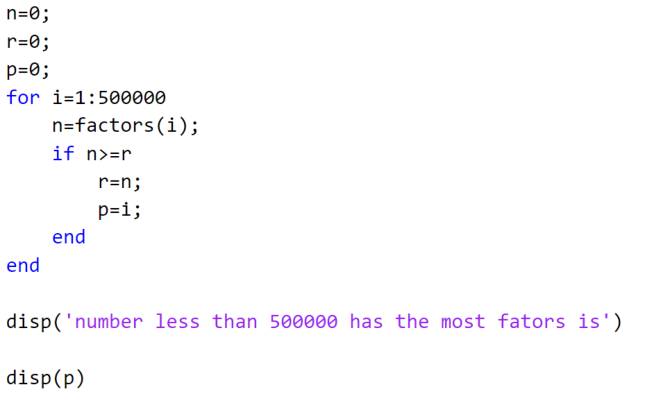
\includepdf[pages={1}]{Picture2.pdf}

\section {Problem 5}
{\bf{Problem: }}
Write a Matlab routine called 'listprimes' that takes as input a positive integer n and outputs a one dimensional array where the ith element is one if i is prime, zero if it is not. Use this function to verify the 6000th prime from question four above. Comment on relative speed.

\subsection{Solution:}

\lstset{language=Matlab,%
    %basicstyle=\color{red},
    breaklines=true,%
    morekeywords={matlab2tikz},
    keywordstyle=\color{blue},%
    morekeywords=[2]{1}, keywordstyle=[2]{\color{black}},
    identifierstyle=\color{black},%
    stringstyle=\color{mylilas},
    commentstyle=\color{mygreen},%
    showstringspaces=false,%without this there will be a symbol in the places where there is a space
    numbers=left,%
    numberstyle={\tiny \color{black}},% size of the numbers
    numbersep=9pt, % this defines how far the numbers are from the text
    emph=[1]{for,end,break},emphstyle=[1]\color{red}, %some words to emphasise
    %emph=[2]{word1,word2}, emphstyle=[2]{style},    
}


\lstinputlisting{listp.m}

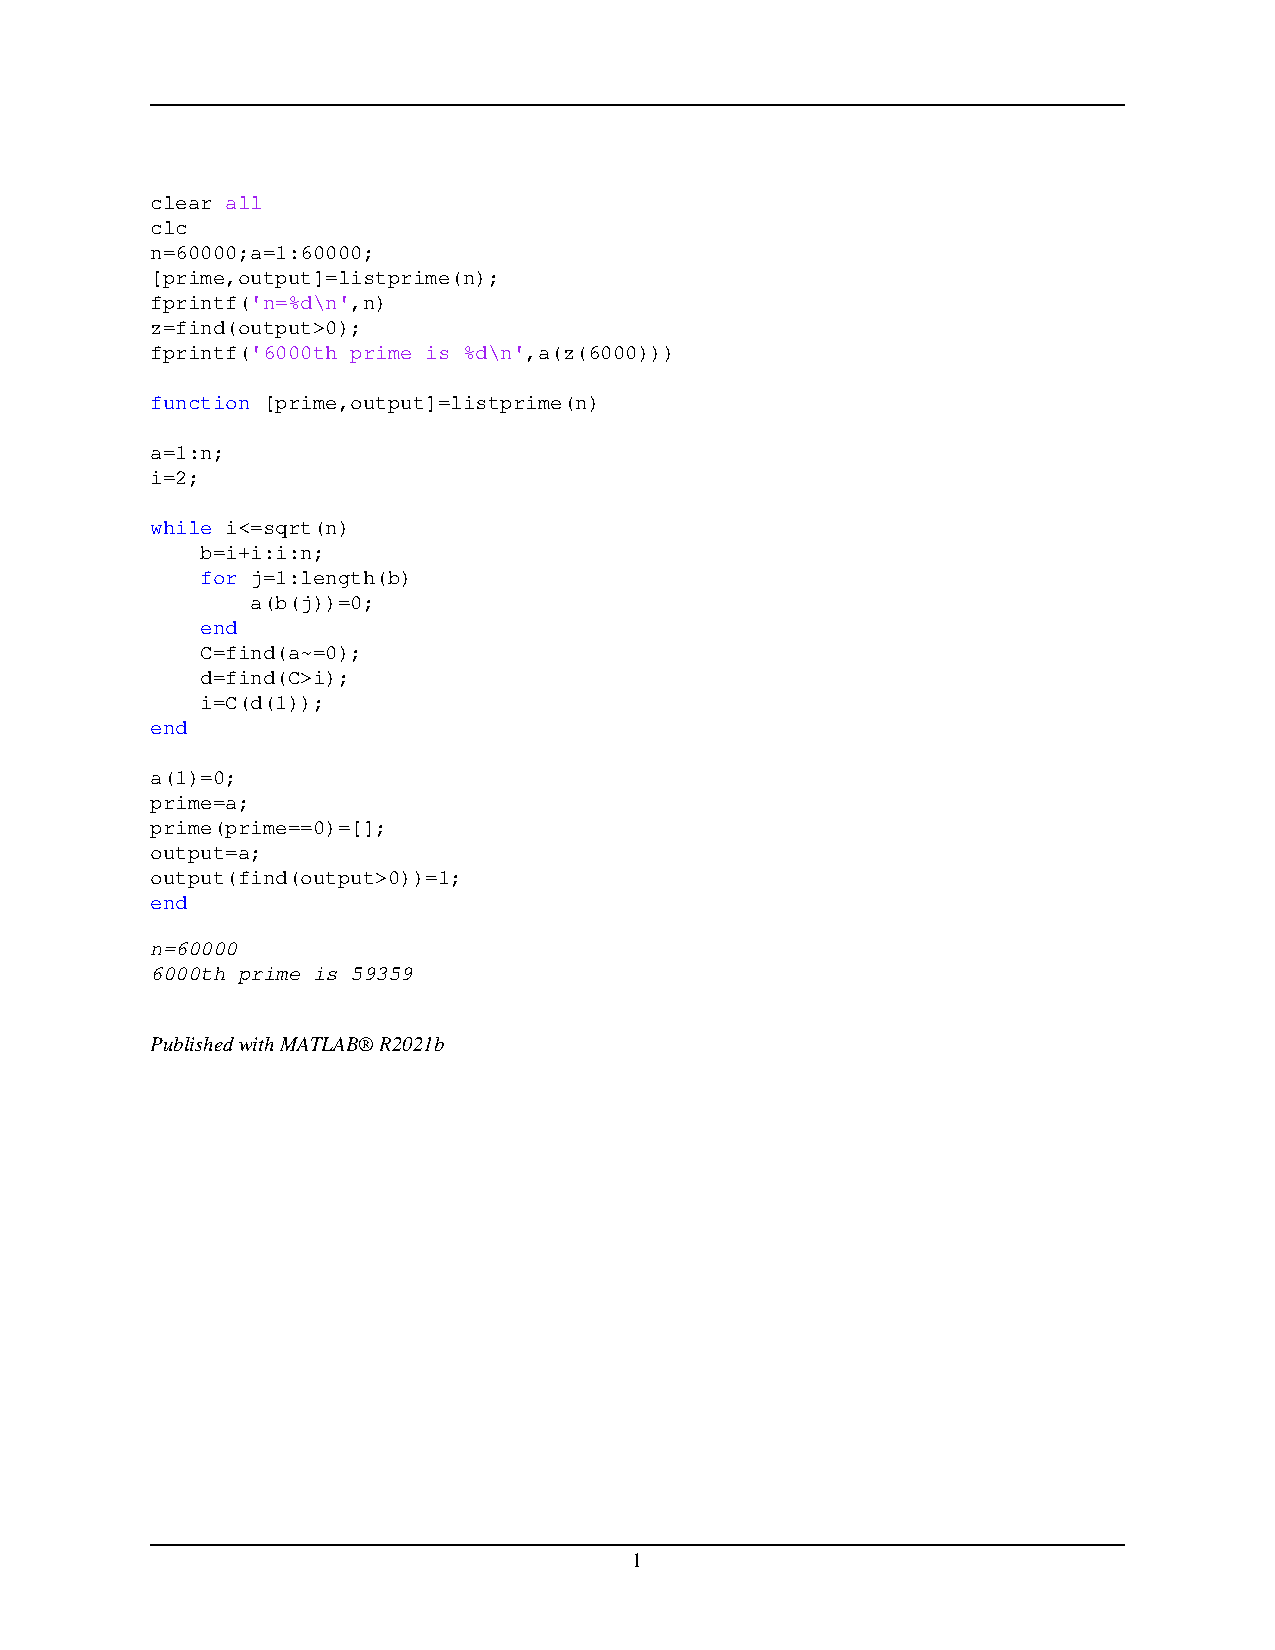
\includepdf[pages={1}]{listp.pdf}


\subsection{Description of solution:}
This problem requires two parts, the first finds primes up to n, the second finds the prime for input value.

\subsection{Results and Conclusions:}
All results from prime function inputs produced reasonable output responses! This indicates the algorithm is performing properly for the problem.
The computation is relatively quick. Answer: the 6000th prime is 59,359.

\section {Problem 6}
{\bf{Problem: }}
Write a Matlab routine called 'listprimes' that takes as input a positive integer n and outputs a one dimensional array where the ith element is one if i is prime, zero if it is not. Use this function to verify the 6000th prime from question four above. Comment on relative speed.

\hfill
\newpage

\subsection{Solution:}
Compared to Problem 2, how can we add loops to utilize factors more effectively?  How much faster is this method and how can we find the most divisors beyond five hundred thousand?

\lstset{language=Matlab,%
    %basicstyle=\color{red},
    breaklines=true,%
    morekeywords={matlab2tikz},
    keywordstyle=\color{blue},%
    morekeywords=[2]{1}, keywordstyle=[2]{\color{black}},
    identifierstyle=\color{black},%
    stringstyle=\color{mylilas},
    commentstyle=\color{mygreen},%
    showstringspaces=false,%without this there will be a symbol in the places where there is a space
    numbers=left,%
    numberstyle={\tiny \color{black}},% size of the numbers
    numbersep=9pt, % this defines how far the numbers are from the text
    emph=[1]{for,end,break},emphstyle=[1]\color{red}, %some words to emphasise
    %emph=[2]{word1,word2}, emphstyle=[2]{style},    
}


\lstinputlisting{max.m}

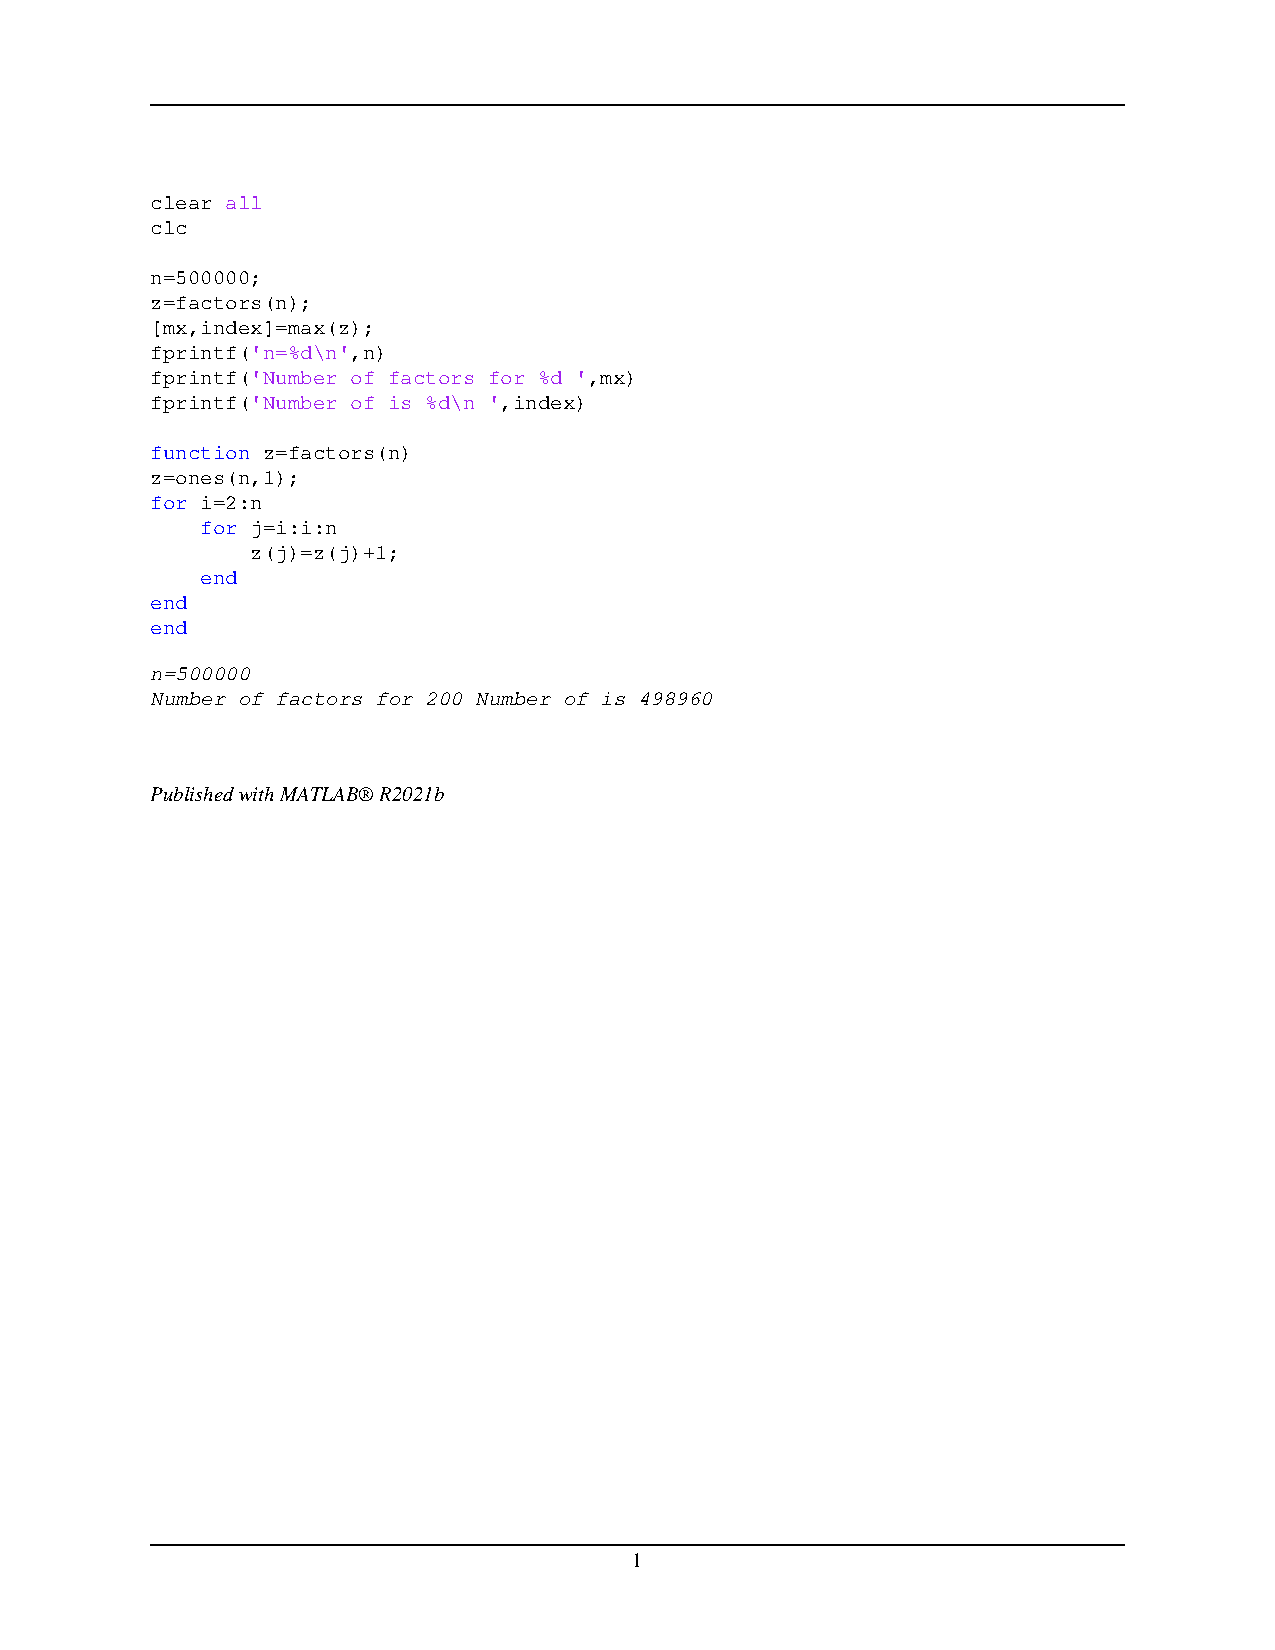
\includepdf[pages={1}]{max.pdf}


\subsection{Description of solution:}
This problem requires an algorithm that utilizes factors  function and two for loops.  The loops find factors up to n.

\subsection{Results and Conclusions:}
All results from factors function inputs produced reasonable output responses! This indicates the algorithm is performing properly for the problem.  
The elapsed time for this method is much faster! By several magnitudes. Answer: Maximum factors can be observed for 200 with number of factors 498,960.

\end{document}